\documentclass[prd,aps,twocolumn,a4paper,showkeys,nofootinbib]{revtex4-2}

\usepackage{amsmath}
\usepackage{amsfonts}
\usepackage{amssymb}	
\usepackage{graphicx}
\usepackage{color}
\usepackage[hidelinks]{hyperref}
\allowdisplaybreaks

\def\TODO{\textcolor{red}{TODO:}}
\def\Mc{{\cal M}_c}

\begin{document}

\title{On NS dataset}

\author{Marina Berbel}

\date{\today}

\maketitle

%==========================================================
\section{Analysis of the raw data}
%==========================================================
Here we do some analysis of the data, without any treatment, just to explore its features.

\subsection{Error in the recovery}
Here we compute the relative error in each quantity as
\begin{equation}
error=\frac{(q_{inj}-q_{rec})}{q_{inj}}.
\end{equation}
Using this there are division by zero in the spins, so we do not show them.  In figure \ref{fig:relative_erros} we can see the results for the train and test dataset. 

The error is bigger for $m_1\leq50$ and $m_2\leq20$. One of the meanings of this is that the BNS will be poorly recovered, making it harder to classify them.

COMMENTS ON EFFECTS OF THIS IN THE REGRESSION?

\begin{figure}[]
  \center
  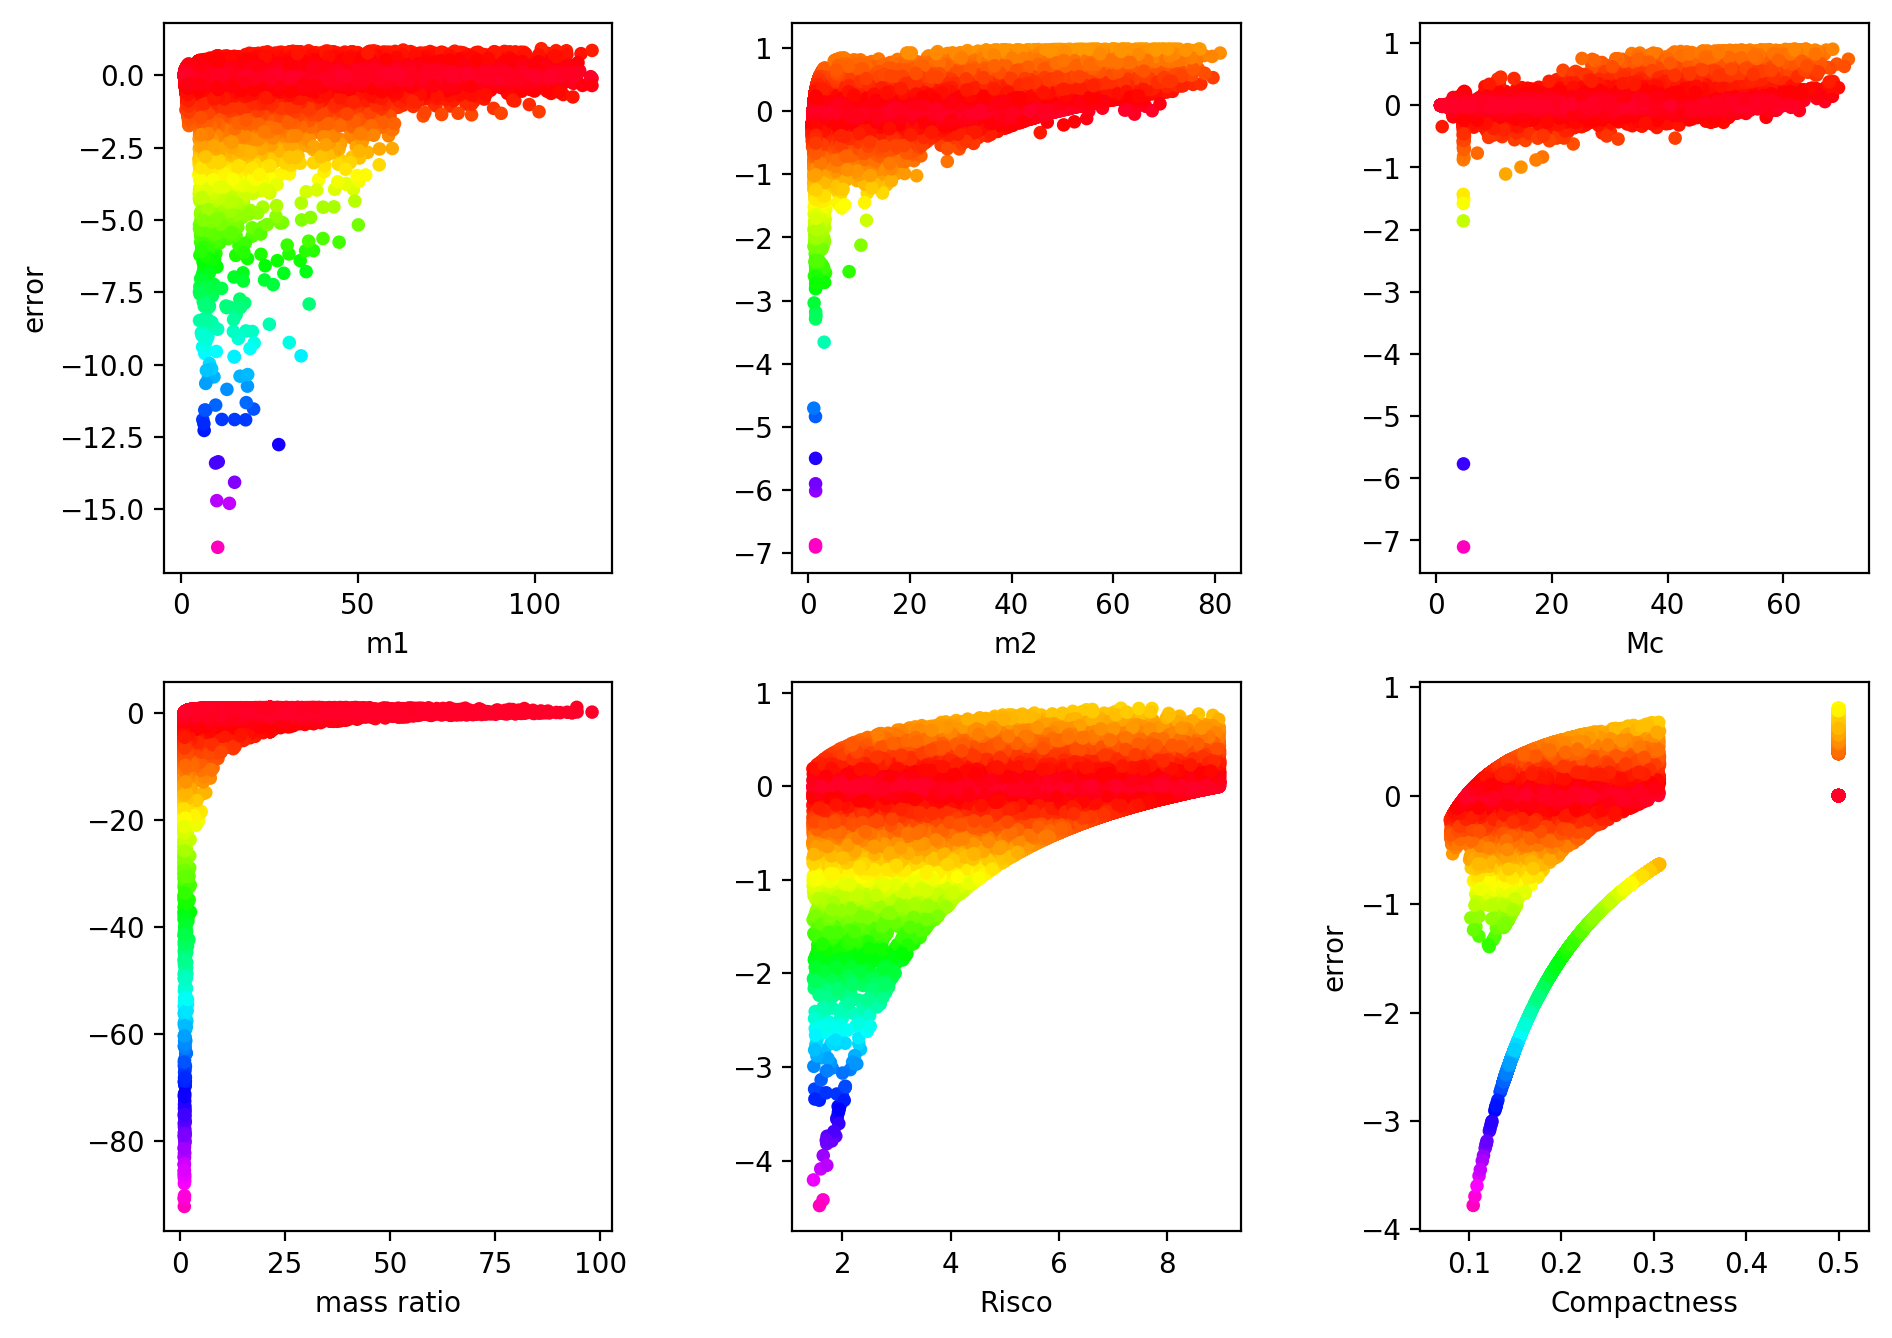
\includegraphics[width=0.45\textwidth]{./FigNS/error_in_train}\\
  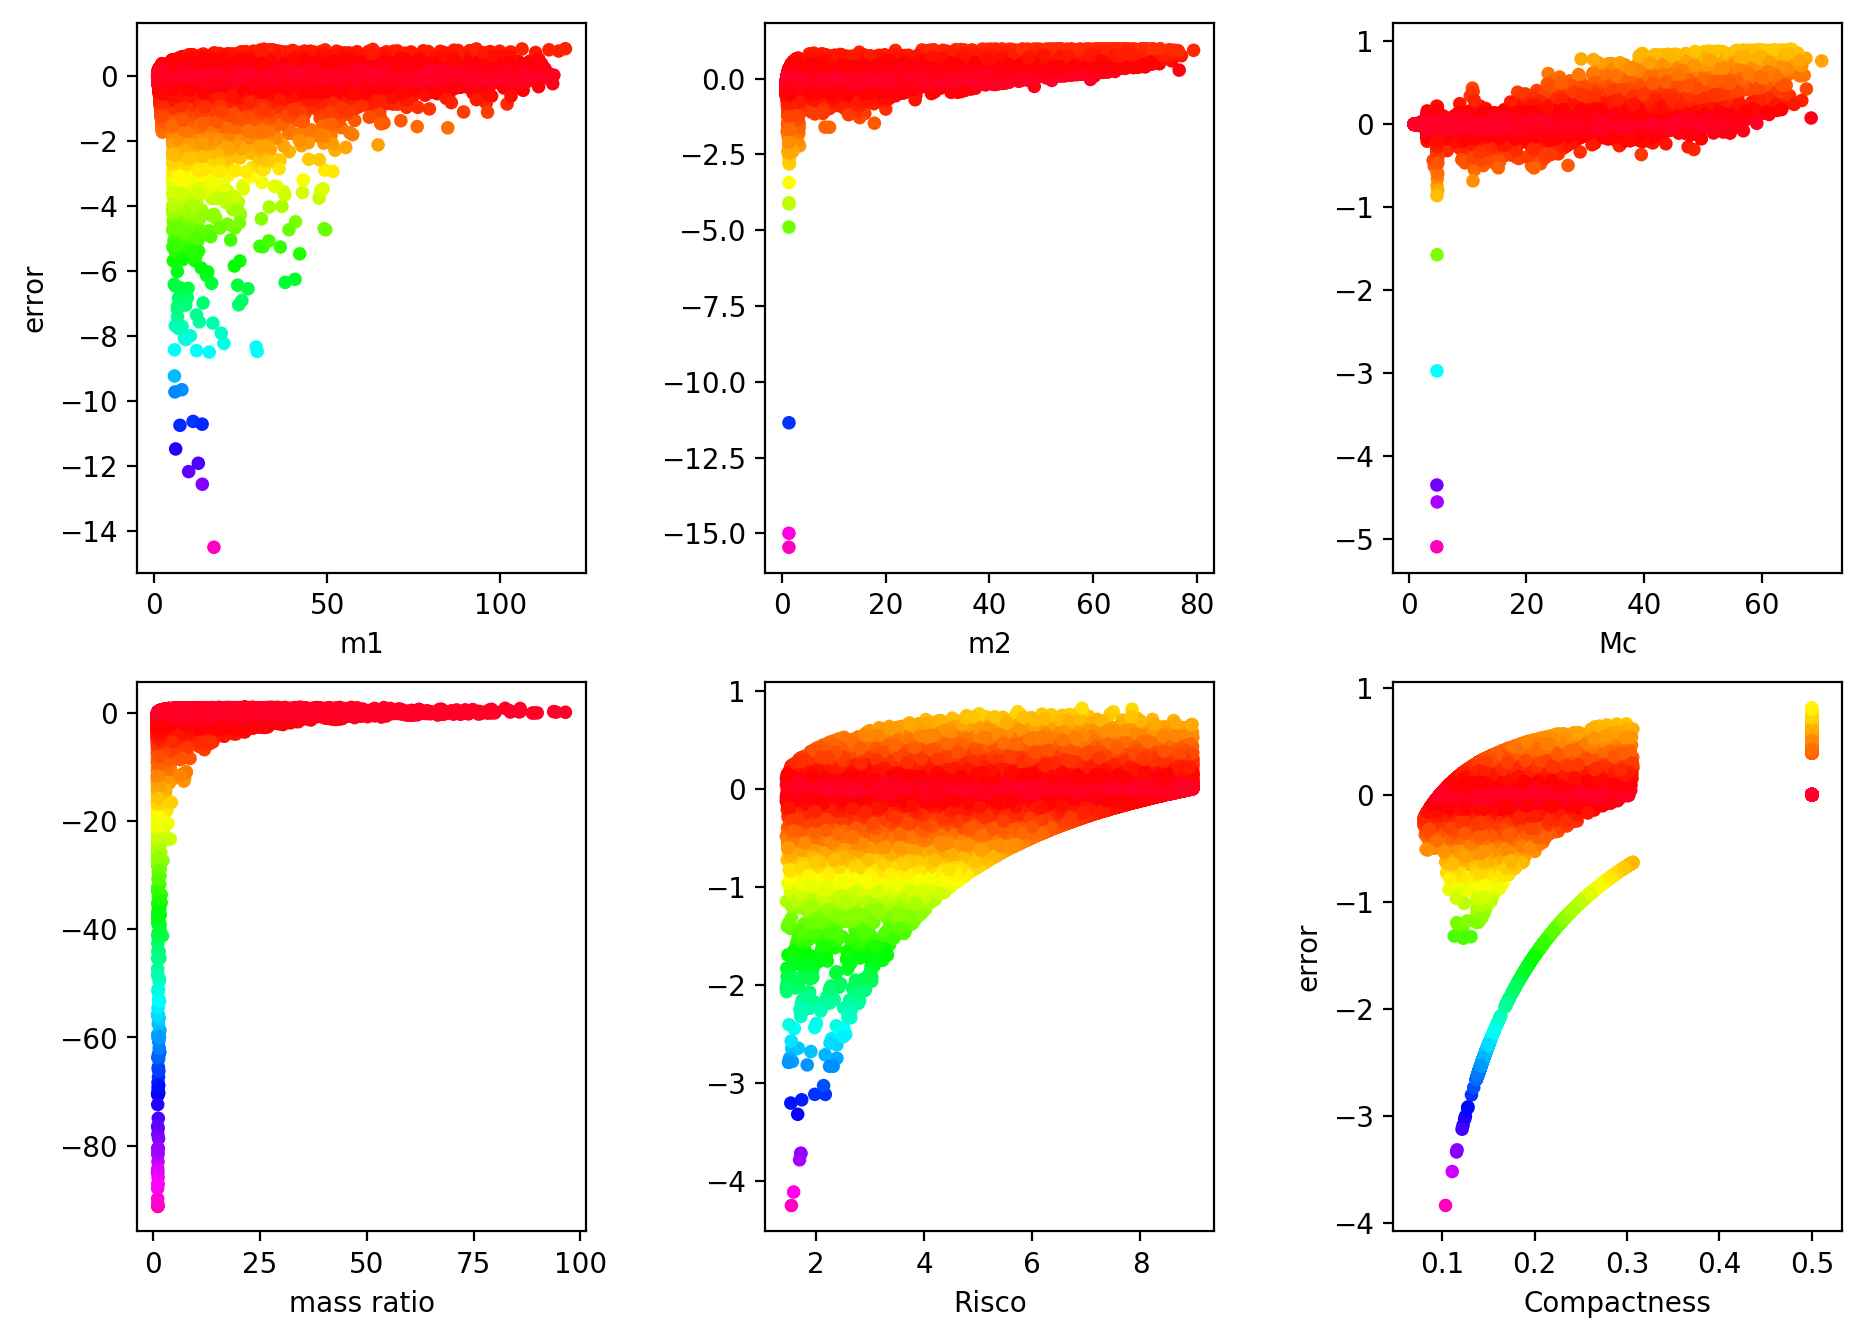
\includegraphics[width=0.45\textwidth]{./FigNS/error_in_test}
  \caption{\label{fig:relative_erros} Relative error in the recovery of each quantity, independent and derived. Top picture: in train dataset. Bottom picture: in test dataset.}
\end{figure}

I also tried to color the plots by SNR, but the range of values is huge (from 8 to 800). In figure \ref{fig:relative_snr} we can see the error of $m_1$ colored by a small range of SNR so we can actually see different colors. It shows that the error does not look dependent on the SNR.

\begin{figure}[]
  \center
  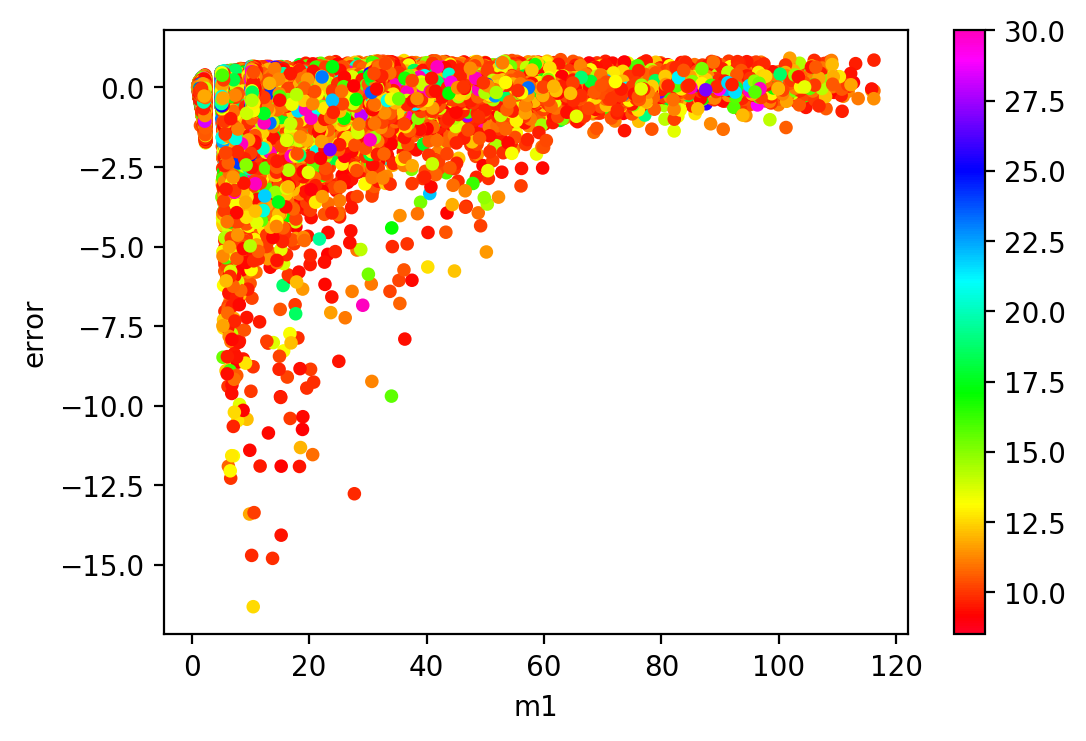
\includegraphics[width=0.45\textwidth]{./FigNS/example_snr}
  \caption{\label{fig:relative_snr} Relative error in the recovery of $m_1$ colored by SNR in a small range to be able to see the different colors.}
\end{figure}

\subsection{Distribution of the label}
We can draw in the $m_1-m_2$ plane the events in the data, colored by their label. This gives us the idea of the function used for labelling and if it will be easy or more difficult to classify the events. Also we can later compare the probability distribution given by the classifier with the actual distribution of the label.

In figure \ref{fig:label_injected} we can see that the event is classified as \textit{HasNS} if $m_2\leq3$.  In figure \ref{fig:label_recovered} we can see that in the data we will use for classification, this is the recovered values of the event from the pipeline, the sharp cut no longer exists because the masses are distorted. We can still observe a dependency on $m_2$ stronger than on $m_1$.

The error in the recovery of $m_2$ will highly affect the classification of events.

\begin{figure}[]
  \center
  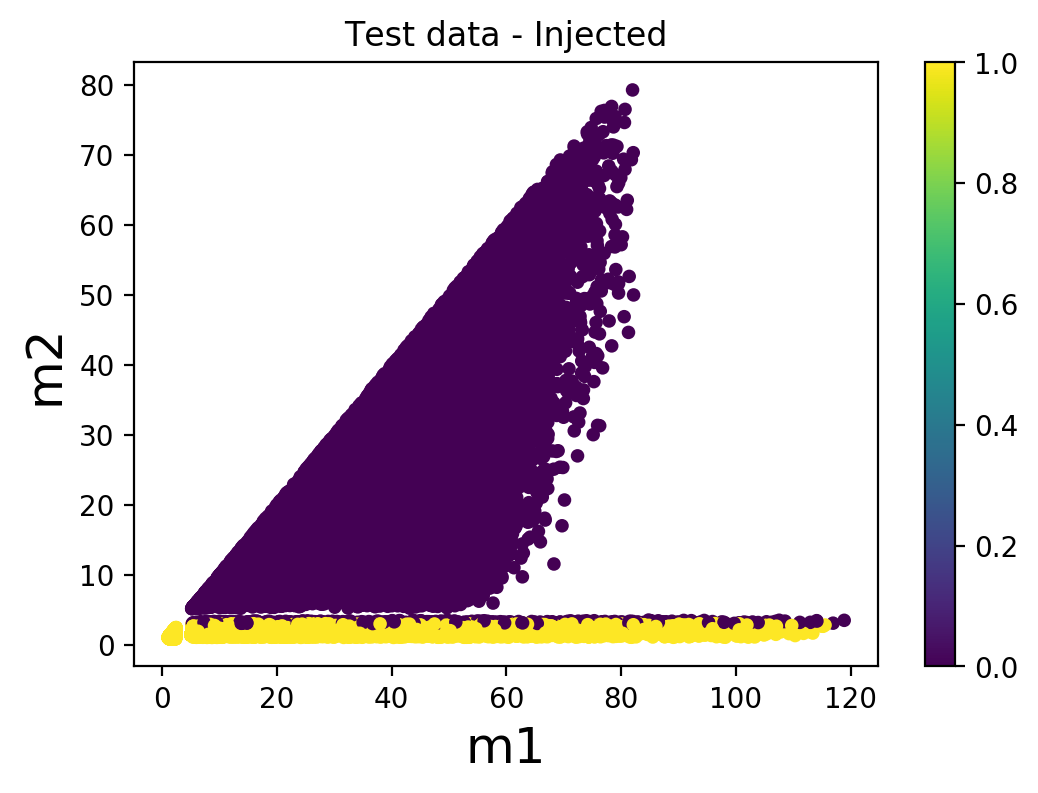
\includegraphics[width=0.3\textwidth]{./FigNS/label_injected}
  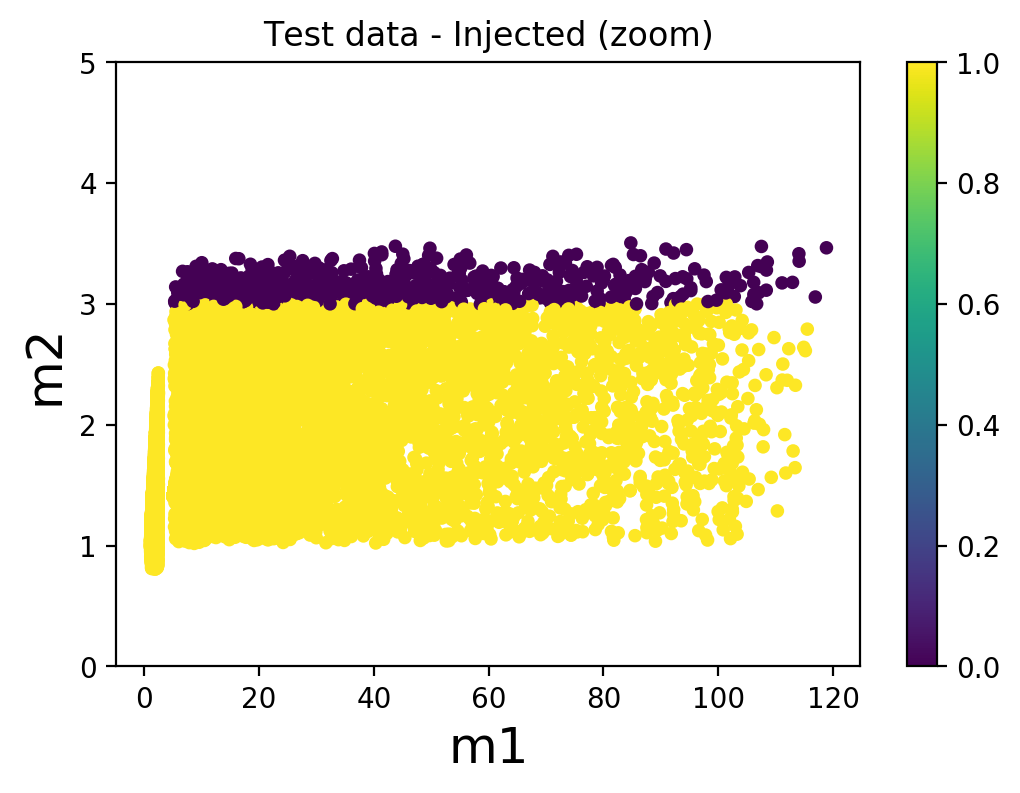
\includegraphics[width=0.3\textwidth]{./FigNS/label_injected_1}
  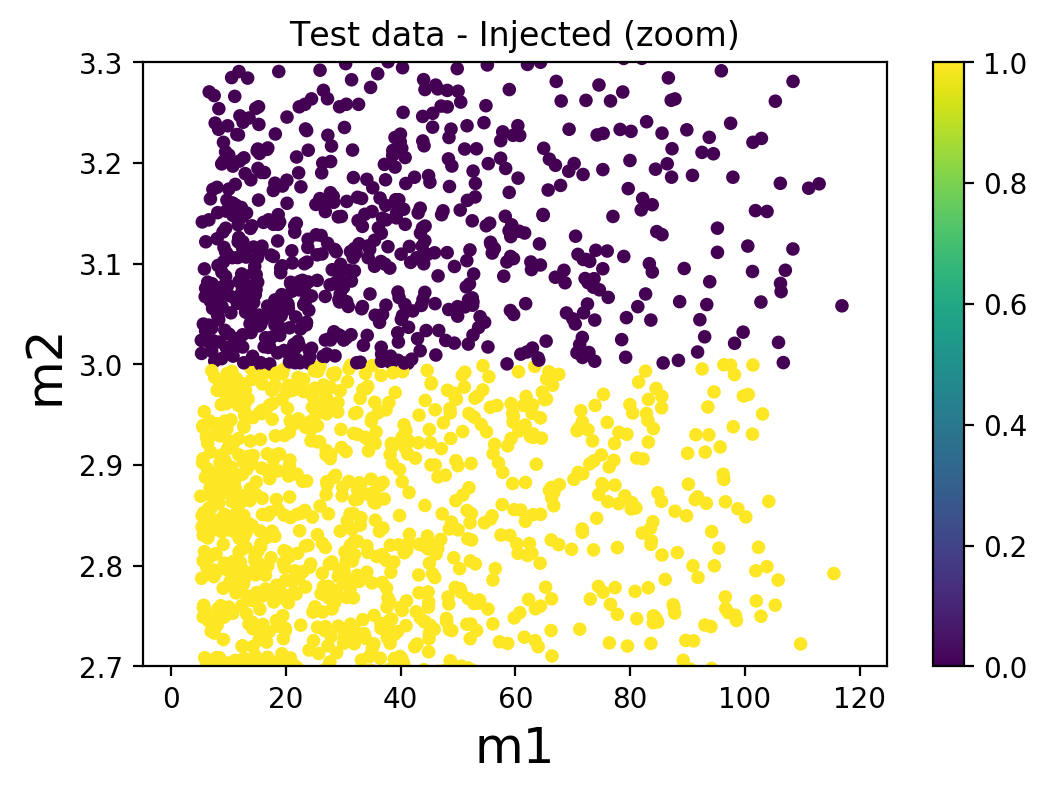
\includegraphics[width=0.3\textwidth]{./FigNS/label_injected_2}
  \caption{\label{fig:label_injected} From the test dataset, injected masses colored by their label. Second and third pictures are zooms of the first one. We can see that there is a sharp cut at $m_2=3$.}
\end{figure}

\begin{figure}[]
  \center
  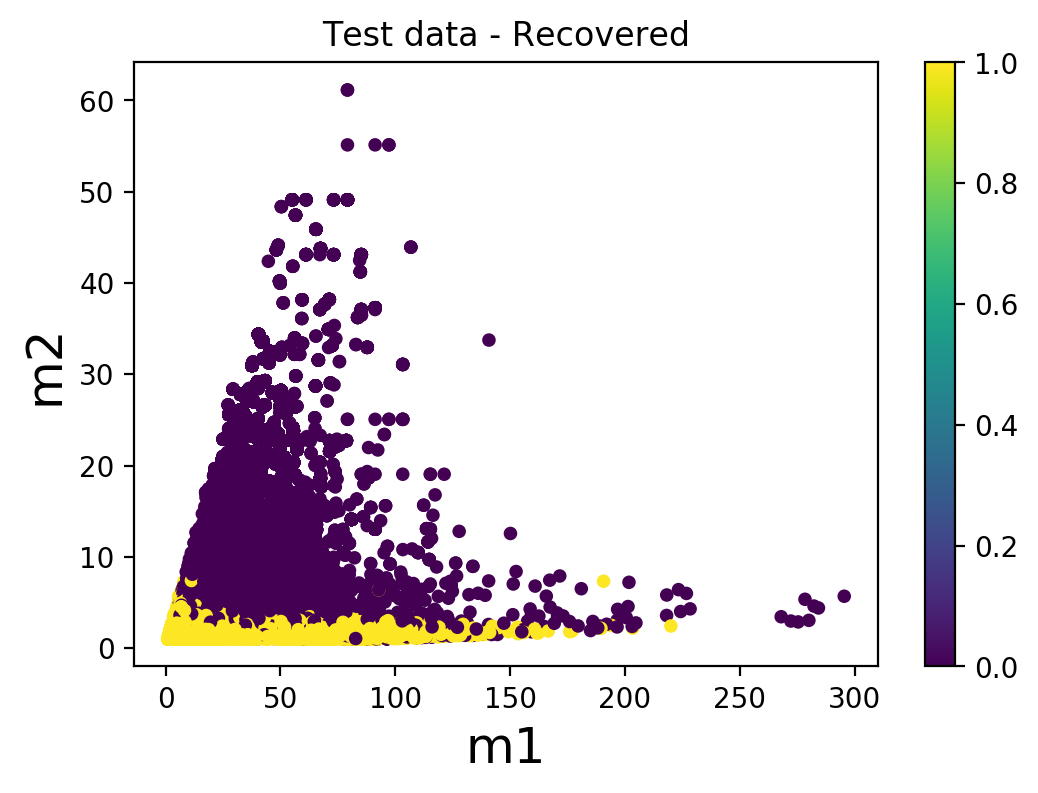
\includegraphics[width=0.3\textwidth]{./FigNS/label_recovered}
  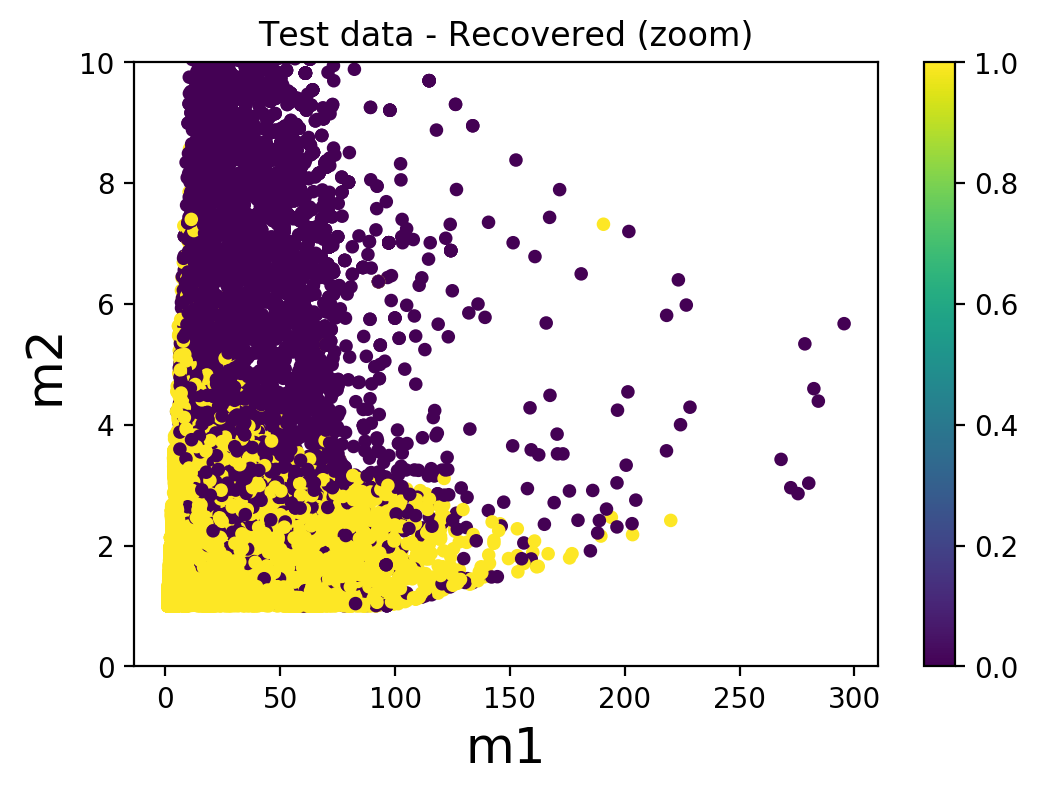
\includegraphics[width=0.3\textwidth]{./FigNS/label_recovered_1}
  \caption{\label{fig:label_recovered} From the test dataset, recovered masses colored by their label. Second picture is a zoom of the first one. The sharp cut is lost in the error of the recovery.}
\end{figure}

Then we also plot the events by the spins of the two bodies, see figure \ref{fig:label_x}. We see that there is another condition here: it is not classified as \textit{hasNS} if $|\chi_2|>0.5$ approximately. This constraint if of course lost in the recovered quantities.

\begin{figure}[]
  \center
  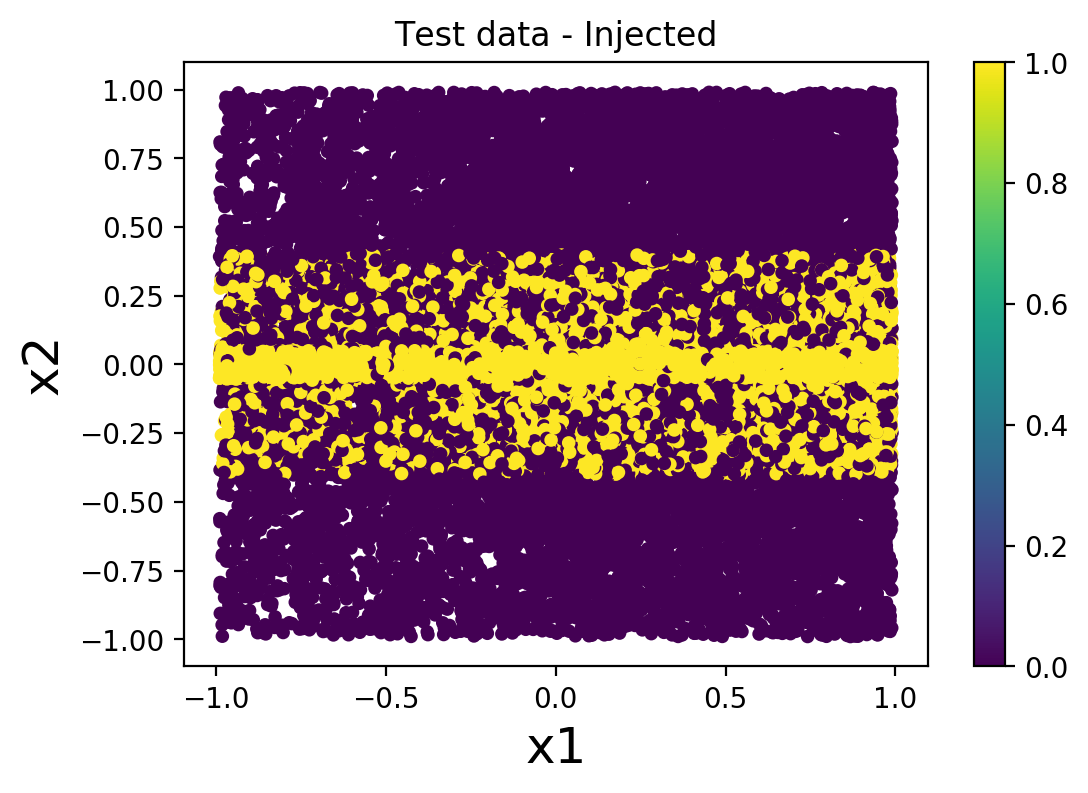
\includegraphics[width=0.3\textwidth]{./FigNS/label_xinjected}
  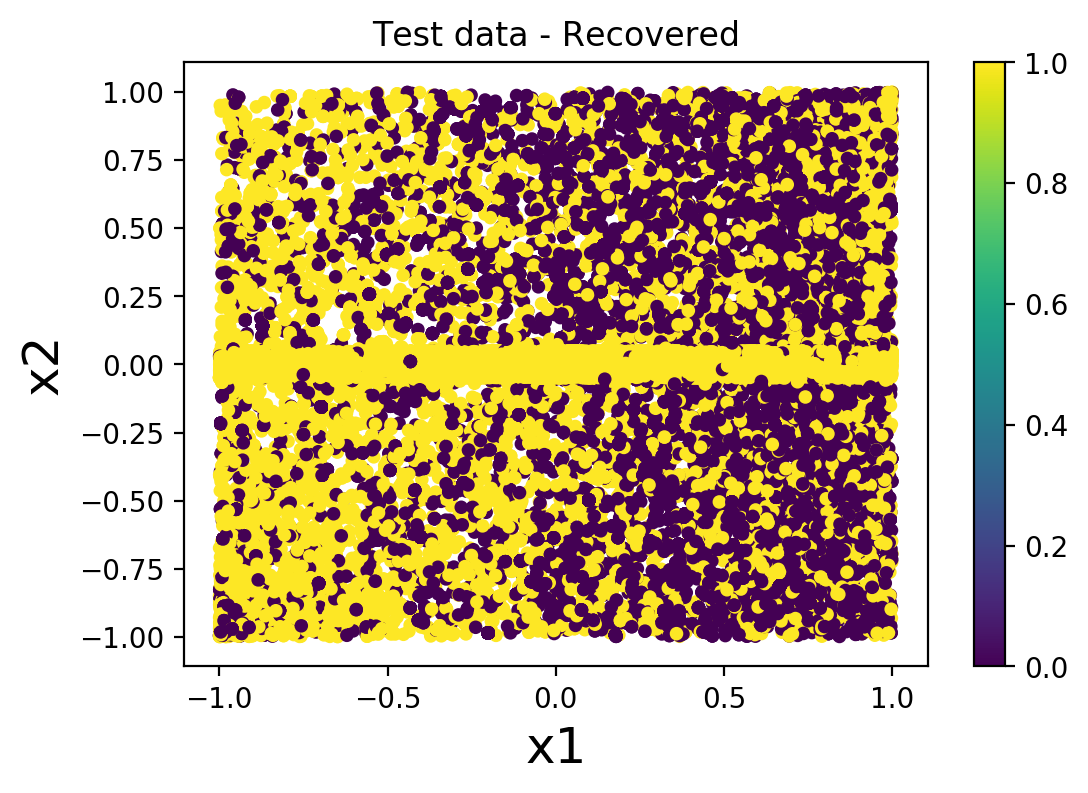
\includegraphics[width=0.3\textwidth]{./FigNS/label_xrecovered}
  \caption{\label{fig:label_x} From the test dataset, injected and recovered spins colored by their label.}
\end{figure}













\end{document}